\documentclass{standalone}
\usepackage{tikz}
\usepackage{verbatim}
\begin{document}
\pagestyle{empty}
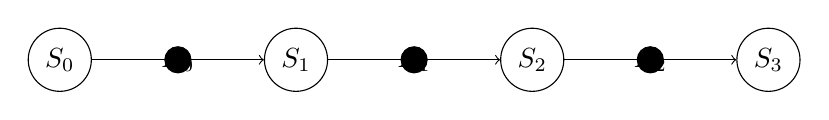
\begin{tikzpicture}
  \foreach \x in {0, 1, 2, 3} {
    \node[draw,circle] (s\x) at (\x*3, 0) {$S_{\x}$};
  }
  \foreach \x in {0, 1, 2} {
    \node[draw,circle,fill] (inter\x) at (\x*3+3/2, 0) {};
    \node  at (\x*3+3/2, 0) {$A_\x$};
  }
  %\node[above right = 1mm of inter0] {$R_{1}$};
  %\node[above right = 1mm of inter1] {$R_{2}$};
  %\node[above right = 1mm of inter2] {$R_{3}$};
  \draw[->] (s0) -- (s1);
  \draw[->] (s1) -- (s2);
  \draw[->] (s2) -- (s3);
  %\node[right = 1mm of s3] {$\ldots$};
\end{tikzpicture}
\end{document}